%!TEX root = ../../root.tex

So far we have focused on one of the possible tasks that deep learning can be used for: regression, i.e. learning a mapping from datapoints in $\mathbb{R}^n$ to other points in $\mathbb{R}^n$, usually simply $\mathbb{R}$, so predicting a value given some \emph{features}.

\emph{Classification} is another very common deep learning task, in which instead we want to predict a \emph{category}, or a \emph{class} for a given datapoint. For example, given some features describing an email, we could be interested to \emph{classify} it as either spam or non-spam; this is an example of \emph{binary classification}. 

One could think that classification is just a special case of regression, since we can represent the set of possible categories as natural numbers, so a subset of $\mathbb{R}$. So the idea would be to use the usual regression and then post-process the output value of the regression in some way. In the previous example of spam detection, by applying a threshold to convert it to a binary output. 

This is not ideal, since we lose some optimality guarantees: while we know that the optimum value returned by linear regression is an optimum, if we do post-processing and convert it to a categorical output the result is not necessarily an optimum anymore.

What we would like to do instead is to modify our loss to more closely reflect our objective, i.e. to minimize directly the error that the model does when predicting the categorical values. As we will see, linearity shows up again.

\paragraph{Logistic regression}

\emph{Logistic regression} is one of the simplest approach to classification.

Let $\{x_i, y_i\}$ be the training data, with $x_i$ being some point in $\mathbb{R}^n$ encoding the features of the $i$-th sample, and $y_i$ being the \emph{label} of the sample, i.e. an encoding of its class. In a binary setting this would mean being a positive or negative sample with respect to some criterion, e.g. being a spam email.
\begin{equation}
    y_i = \begin{cases}
        0 & x_i \text{ is a negative sample} \\
        1 & x_i \text{ is a positive sample}
    \end{cases}
\end{equation}

In this setting, we define a new model
\begin{equation}
    \hat{f}(x_i) = \underbrace{ax_i + b}_\text{linear}
\end{equation}
that makes class \emph{predictions} as follows
\begin{equation}
    \hat{y}_i = \begin{cases}
        0 & \sigma(\hat{f}(x_i)) \leq 0.5 \\
        1 & \sigma(\hat{f}(x_i)) > 0.5 \\
    \end{cases}
\end{equation}
and a new loss
\begin{equation}
	\ell_\mathbf{\Theta}(\{x_i, y_i\}) = \sum_{i=1}^{n}\left( y_i - \sigma(ax_i + b) \right)^2.
\end{equation}

Notice that both the model and the loss are very similar to the regression setting, with the difference that we introduced thresholding and $\sigma(\cdot)$, that is a function called \emph{logistic sigmoid}, defined as follows:
\begin{equation}
	\sigma(x) = \frac{1}{1+e^{-x}}.
\end{equation}
The logistic sigmoid squashes the real line to within the values $0$ and $1$ (this is called \emph{saturation} effect) as we can see below:
\begin{figure}[H]
	\centering
	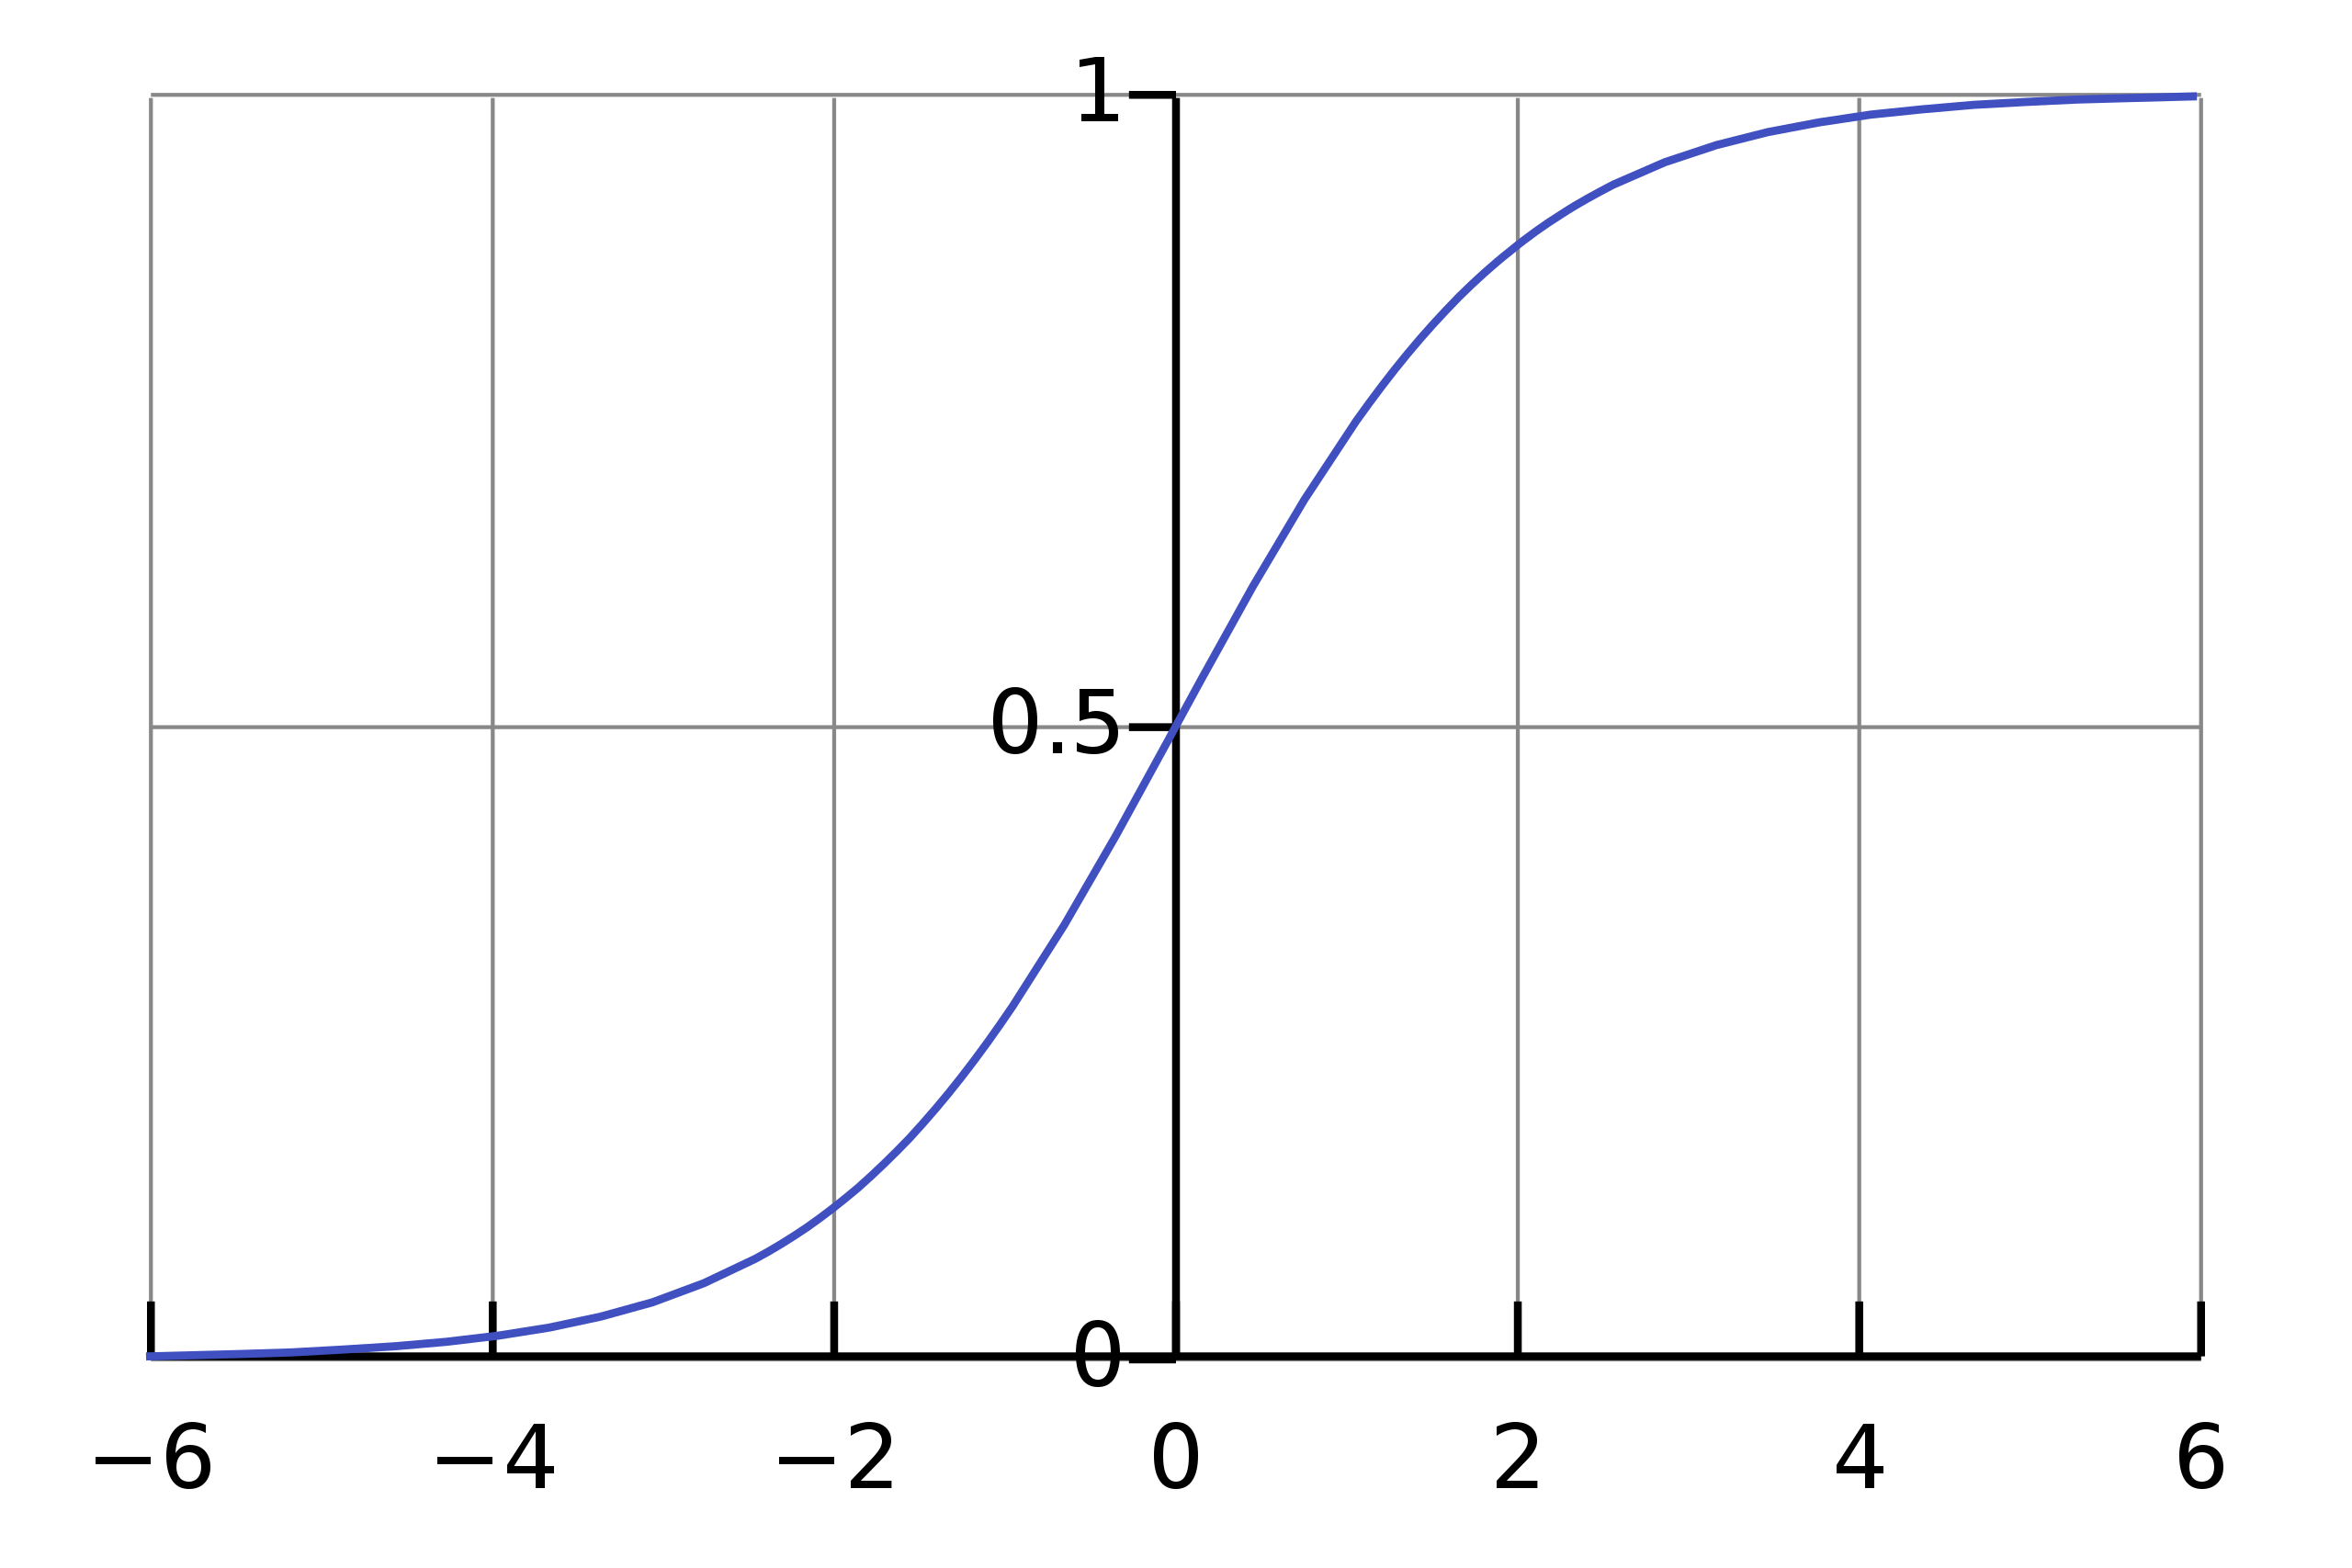
\includegraphics[width=.3\textwidth]{05/sigmoid}
	\caption{Logistic sigmoid.}\label{fig:sigmoid}	
\end{figure}
We like this property of the sigmoid, since as we have seen $y_i$ will take values in $\{0, 1\}$, and therefore we can compare numerically the labels and the model output: the loss is close to zero over samples for which the label is $0$ and the model correctly outputs values close to $0$ but also samples for which the label is $1$ and the model correctly outputs values close to $1$.

There is a drawback however: notice that the sigmoid is clearly nonlinear, and even worse non-convex, thus making the whole loss function non-convex. We cannot just take the gradient, set it to $0$ and solve for $a$ and $b$: we don't have any optimality guarantee. Therefore, we can either try to minimize a non convex function or we can try to come up with a different loss. 

The modified loss is as follows:
\begin{equation}
	\ell_\mathbf{\Theta}(\{x_i, y_i\}) = \sum_{i=1}^{n}c(x_i, y_i)
\end{equation}
where
\begin{equation}
	c(x_i, y_i) = \begin{cases}
               		-ln(\sigma(ax_i+b)),        & y_i = 1\\
               		-ln(1 - \sigma(ax_i+b)),    & y_i = 0
            	  \end{cases}
\end{equation}
is convex. To prove it, we should either prove that the Jensen's inequality holds, or directly show that its second derivative is always non-negative (the actual definition of convex function). In this case we have
\begin{align}
    \dv{x} \left[-ln(\sigma(x))\right] & = \dv{x} \left[-ln\left(\frac{1}{1 + e^{-x}}\right) \right] = \dv{x} \left[ -(ln(1) - ln(1+e^{-x})) \right] = \dv{x} \left[ ln(1+e^{-x}) \right] \\
    & = -\frac{e^{-x}}{1 + e^{-x}} = -\frac{-1 + 1 + e^{-x}}{1 + e^{-x}} = -1 + \frac{1}{1 + e^{-x}} = -1 + \left( 1 + e^{-x} \right)^{-1} \\
    \dv[2]{x} \left[ -ln(\sigma(x)) \right] & = \dv{x} \left[ -1 + \left( 1 + e^{-x} \right)^{-1} \right] \\ 
    & = -( 1 + e^{-x})^{-2} (-e^{-x}) = \frac{e^{-x}}{(1 + e^{-x})^2} \geq 0
\end{align}
so the function is indeed convex. In a similar fashion we could prove that also $-ln(1 - \sigma(x))$ is convex so overall $c(x_i, y_i)$ is convex.

Bringing all together we have 
\begin{equation}
	c(x_i, y_i) = -y_i ln(\sigma(ax_i+b)) - (1 - y_i)ln(1 - \sigma(ax_i+b)).
\end{equation}
since the first term will be present only when $y_i = 1$ and the second only when $y_i = 0$, as per the definition of $c(x_i, y_i)$, and thus we have the following expression for the loss:
\begin{equation}
	\ell_\mathbf{\Theta}(\{x_i, y_i\}) = - \sum_{i=1}^{n} \left( y_iln(\sigma(ax_i+b)) + (1 - y_i)ln(1 - \sigma(ax_i+b)) \right).
\end{equation}

To find a solution we compute the gradient and set it to zero, therefore we obtain:
\begin{align}
	\nabla_\Theta \sum_{i=1}^{n} \left( y_iln(\sigma(ax_i+b)) + (1 - y_i)ln(1 - \sigma(ax_i+b)) \right) &= 0 \\
	\sum_{i=1}^{n} \nabla_\Theta \left( y_iln(\sigma(ax_i+b)) + (1 - y_i)ln(1 - \sigma(ax_i+b)) \right) &= 0 \\
	\sum_{i=1}^{n} \left( \nabla_\Theta y_iln(\sigma(ax_i+b)) + \nabla_\Theta (1 - y_i) ln(1 - \sigma(ax_i+b)) \right) &= 0 \\
	\sum_{i=1}^{n} \left( y_i \nabla_\Theta ln(\sigma(ax_i+b)) + (1 - y_i) \nabla_\Theta ln(1 - \sigma(ax_i+b)) \right) &= 0 
\end{align}

In the following, we are going to need the derivative of the sigmoid, which we now derive:
\begin{align}
	\partfrac{\sigma(x)}{x} &= \partfrac{}{x} \frac{1}{1 + e^{-x}} = \frac{e^{-x}}{\left(1 + e^{-x}\right)^2} = \frac{1}{ 1 + e^{-x}} \cdot \frac{e^{-x}}{ 1 + e^{-x}} \\
	&=\frac{1}{ 1 + e^{-x}} \cdot \frac{(1 + e^{-x}) - 1}{1 + e^{-x}} = \frac{1}{ 1 + e^{-x}} \cdot \left( 1 - \frac{1}{1 + e^{-x}} \right) \\
	&= \sigma(x) \cdot \left( 1 - \sigma(x) \right) \label{eq:der-sig}
\end{align}

Consider the first gradient
\begin{equation}
	\nabla_\Theta \underbrace{ln(\sigma(ax_i+b))}_{f(g(h(\Theta)))}
\end{equation}
to compute the derivative of a composed function we can apply the \emph{chain rule} to each partial derivative
\begin{equation}
	\frac{\partial}{\partial a}f(g(h(a, b))) = \frac{\partial f}{\partial g} \cdot \frac{\partial g}{\partial h} \cdot \frac{\partial h}{\partial a}
\end{equation}
replacing it on our fist gradient we have that
\begin{align}
	\frac{\partial}{\partial a}f(g(h(a, b))) &= \frac{\partial f}{\partial g} \cdot \frac{\partial g}{\partial h} \cdot \frac{\partial}{\partial a}(ax_i + b) \\
	&= \frac{\partial f}{\partial g} \cdot \frac{\partial g}{\partial h} \cdot x_i \\
	&= \frac{\partial f}{\partial g} \cdot \frac{\partial}{\partial (ax_i+b)}\sigma(ax_i+b) \cdot x_i 
\end{align}
Now, recalling the derivative of the sigmoid \cref{eq:der-sig}
\begin{align}
	\frac{\partial}{\partial a}f(g(h(a, b))) &= \frac{\partial ln(\sigma(ax_i+b))}{\partial \sigma(ax_i+b)} \cdot \sigma(ax_i+b) \cdot \left( 1 - \sigma(ax_i+b) \right) \cdot x_i \\
	&= \frac{1}{\sigma(ax_i+b)} \cdot \sigma(ax_i+b) \cdot \left( 1 - \sigma(ax_i+b) \right) \cdot x_i \\
	&= \left( 1 - \sigma(ax_i+b) \right) \cdot x_i
\end{align}
and we should continue with the other parameters and considering all terms of the previous expression, but we immediately see that the parameters enter the gradient in a \emph{nonlinear} way since we have the logistic sigmoid which is not a linear transformation.
In particular our gradient $\nabla_\Theta\ell_\Theta$ is a \emph{transcendental} equation (\textit{i.e.} some transcendental function\footnote{If the function is not a finite series we call it a transcendental function} appears in the expression, in our case the exponential inside the sigmoid is the transcendental function) and can be proven that for this kind of equations no analytical solution can be found. So to find a solution we are going to do \emph{nonlinear} optimization.